\chapter{Desenvolvimento do Projeto}

Nesta seção são detalhadas as tecnologias, ferramentas e práticas adotadas para o desenvolvimento do aplicativo Linha Vital, contemplando desde a definição das regras de negócio até os testes de qualidade que asseguram o pleno funcionamento da solução.

O capítulo apresenta os elementos que nortearam a construção do sistema, incluindo o escopo do projeto, requisitos, histórias de usuário, arquitetura da solução, tecnologias empregadas, estratégias de testes, aspectos de segurança da informação e a modelagem do banco de dados.

\section{Escopo do Projeto}

O objetivo central do projeto é desenvolver um aplicativo mobile voltado ao auxílio emergencial e à verificação de atividade de pessoas idosas, indivíduos com necessidades especiais e pessoas que vivem sozinhas.

O sistema foi concebido para monitorar períodos de inatividade do usuário por meio de notificações e solicitações periódicas de confirmação de atividade, além de oferecer recursos de acionamento emergencial integrados às funcionalidades de acessibilidade do dispositivo móvel.

Em situações de alerta, o aplicativo deve enviar notificações automáticas a contatos de confiança e contatos de emergência previamente cadastrados, ampliando a rede de suporte em casos críticos.

Com base na fundamentação teórica e nos estudos realizados sobre o cenário atual e seus desafios, foram estabelecidas regras de negócio que orientam a filosofia e o funcionamento do aplicativo. A partir dessas regras, foram definidos requisitos funcionais e não funcionais, traduzindo o escopo conceitual em especificações técnicas implementáveis.

Essa abordagem assegura que o produto final esteja alinhado às necessidades do público-alvo, garantindo simplicidade, acessibilidade e confiabilidade.


\subsection{Regras de negócio}

As regras de negócio definem os comportamentos, restrições e condições que orientam o funcionamento do sistema Linha Vital. Elas foram elaboradas com base nos requisitos identificados durante o levantamento de necessidades dos usuários e servem como referência para a definição dos requisitos funcionais e não funcionais da aplicação.

Os Quadros~\ref{quad_rn1} e~\ref{quad_rn2} apresentam as regras de negócio estabelecidas para o sistema.

\begin{table}[H]
\caption{Regras de negócio do sistema Linha Vital (Parte 1)}
\label{quad_rn1}
\centering

\begin{tabular}{|c|p{4cm}|p{8cm}|}
\hline
\textbf{ID} & \textbf{Nome} & \textbf{Descrição} \\
\hline

RN01 & Cadastro mínimo obrigatório &
O sistema deve exigir o cadastro de pelo menos um contato de emergência e um contato de confiança antes da ativação do monitoramento. \\
\hline

RN02 & Classificação e gerenciamento de contatos &
Os contatos devem ser classificados como emergência ou confiança, permitindo múltiplos contatos por categoria e exigindo pelo menos um meio de contato válido. \\
\hline

RN03 & Parametrização de inatividade &
O usuário deve definir o tempo máximo de inatividade, o intervalo entre notificações e a quantidade máxima de tentativas de verificação. \\
\hline

RN04 & Critério de atividade do usuário &
O sistema deve considerar o usuário ativo quando houver interação com o dispositivo, resposta a notificações ou desbloqueio do aparelho. \\
\hline

RN05 & Monitoramento não invasivo &
O sistema não deve coletar dados sensíveis como áudio, vídeo ou biometria sem consentimento, utilizando apenas sinais indiretos de atividade. \\
\hline

RN06 & Envio de notificações periódicas &
O sistema deve enviar notificações em intervalos definidos para solicitar confirmação de bem-estar do usuário. \\
\hline

RN07 & Confirmação de bem-estar &
O usuário deve confirmar seu estado por meio de interação no aplicativo, notificação ou recurso de acessibilidade. \\
\hline

RN08 & Escalonamento de notificações &
O sistema deve realizar múltiplas tentativas de contato com o usuário, respeitando intervalos e limites configurados. \\
\hline

RN09 & Condição de emergência &
Uma situação de emergência deve ser caracterizada quando o tempo de inatividade for excedido e não houver resposta após as tentativas de verificação. \\
\hline

RN10 & Princípio de segurança preventiva &
Na ausência de confirmação do usuário, o sistema deve assumir risco potencial e acionar o protocolo de emergência. \\
\hline

RN11 & Conteúdo do alerta &
Todo alerta deve conter identificação do usuário, data e hora do evento, tipo de acionamento e última localização conhecida, quando disponível. \\
\hline

\end{tabular}

\legend{Fonte: Elaborado pelos autores.}
\end{table}

\begin{table}[H]
\caption{Regras de negócio do sistema Linha Vital (Parte 2)}
\label{quad_rn2}
\centering

\begin{tabular}{|c|p{4cm}|p{8cm}|}
\hline
\textbf{ID} & \textbf{Nome} & \textbf{Descrição} \\
\hline

RN12 & Ordem de acionamento de contatos &
O sistema deve acionar primeiro os contatos de confiança e, após um intervalo definido, os contatos de emergência. \\
\hline


RN13 & Escalonamento entre contatos &
Caso não haja resposta, o sistema deve acionar outros contatos disponíveis respeitando a ordem definida. \\
\hline

RN14 & Confirmação de recebimento &
O sistema deve considerar um alerta como atendido quando um contato confirmar o recebimento da notificação. \\
\hline

RN15 & Acionamento manual de emergência &
O usuário deve poder acionar manualmente um alerta de emergência a qualquer momento. \\
\hline

RN16 & Integração de acessibilidade &
O sistema deve permitir acionamento de emergência por interface do aplicativo, botões físicos ou recursos de acessibilidade do dispositivo. \\
\hline

RN17 & Cancelamento pré-envio &
O usuário pode cancelar o alerta antes que ele seja enviado aos contatos. \\
\hline

RN18 & Cancelamento pós-envio &
O sistema deve permitir envio de notificação de cancelamento aos contatos em caso de falso alarme. \\
\hline

RN19 & Encerramento da ocorrência &
Uma ocorrência deve ser encerrada quando o usuário cancelar o alerta ou quando um contato confirmar atendimento. \\
\hline

RN20 & Estados do sistema &
O sistema deve operar com estados definidos: inativo, ativo, aguardando confirmação, em alerta e emergência acionada. \\
\hline

RN21 & Autonomia do usuário &
O usuário deve poder ativar ou desativar o monitoramento a qualquer momento. \\
\hline

RN22 & Tratamento de falhas de comunicação &
O sistema deve tentar reenviar notificações em caso de falha e utilizar canais alternativos quando disponíveis. \\
\hline

RN23 & Minimização de falsos positivos &
O sistema deve reduzir alertas indevidos por meio de múltiplas tentativas de confirmação e parâmetros configuráveis. \\
\hline

RN24 & Proteção de dados &
O sistema deve garantir a segurança e privacidade dos dados conforme a legislação vigente (LGPD). \\
\hline

\end{tabular}

\legend{Fonte: Elaborado pelos autores.}
\end{table}


\subsection{Requisitos funcionais}

Os requisitos funcionais descrevem as funcionalidades que devem ser implementadas pelo sistema Linha Vital para atender às necessidades dos usuários e às regras de negócio estabelecidas. Esses requisitos especificam os comportamentos esperados da aplicação, contemplando desde o cadastro e monitoramento dos usuários até os mecanismos de alerta e comunicação em situações de emergência.

Os Quadros~\ref{quad_rf1} e~\ref{quad_rf2} apresentam os requisitos funcionais definidos para o sistema.

\begin{table}[H]
\caption{Requisitos Funcionais (Parte 1)}
\label{quad_rf1}
\centering
\begin{tabular}{|c|p{8cm}|c|}
\hline
\textbf{ID} & \textbf{Descrição} & \textbf{Relação RF/RN} \\
\hline
RF01 & O sistema deve permitir o cadastro de usuários. & RN01 \\
\hline
RF02 & O sistema deve permitir o cadastro de contatos de emergência e contatos de confiança. & RN01, RN02 \\
\hline
RF03 & O sistema deve impedir a ativação do monitoramento sem o cadastro mínimo de contatos. & RN01 \\
\hline
RF04 & O sistema deve permitir a edição e remoção de contatos cadastrados. & RN02 \\
\hline
RF05 & O sistema deve permitir ao usuário configurar o tempo máximo de inatividade, intervalo entre notificações e número de tentativas. & RN03 \\
\hline
RF06 & O sistema deve monitorar a atividade do usuário com base em interações no dispositivo, desbloqueio e resposta a notificações. & RN04 \\
\hline
RF07 & O sistema deve enviar notificações periódicas de verificação de bem-estar. & RN06 \\
\hline
RF08 & O sistema deve permitir que o usuário confirme seu estado por meio de interação com a notificação, aplicativo ou recursos de acessibilidade. & RN07 \\
\hline
RF09 & O sistema deve realizar múltiplas tentativas de notificação respeitando intervalos e limites configurados. & RN08 \\
\hline
RF10 & O sistema deve identificar automaticamente uma situação de emergência com base na inatividade e ausência de resposta. & RN09, RN10 \\
\hline
RF11 & O sistema deve enviar alertas automáticos aos contatos cadastrados em caso de emergência. & RN11 \\
\hline
RF12 & O sistema deve incluir no alerta informações como identificação do usuário, data/hora, tipo de acionamento e localização quando disponível. & RN11 \\
\hline
RF13 & O sistema deve seguir uma ordem de prioridade no acionamento dos contatos. & RN12 \\
\hline

\end{tabular}

\legend{Fonte: Elaborado pelos autores.}
\end{table}

\begin{table}[H]
\caption{Requisitos Funcionais (Parte 2)}
\label{quad_rf2}
\centering
\begin{tabular}{|c|p{8cm}|c|}
\hline
\textbf{ID} & \textbf{Descrição} & \textbf{Relação RF/RN} \\
\hline
RF14 & O sistema deve escalar o acionamento para múltiplos contatos caso não haja resposta inicial. & RN13 \\
\hline
RF15 & O sistema deve permitir que contatos confirmem o recebimento do alerta. & RN14 \\
\hline
RF16 & O sistema deve permitir o acionamento manual de emergência pelo usuário. & RN15 \\
\hline
RF17 & O sistema deve permitir acionamento de emergência por meio de recursos de acessibilidade do dispositivo. & RN16 \\
\hline
RF18 & O sistema deve permitir o cancelamento de um alerta antes do envio. & RN17 \\
\hline
RF19 & O sistema deve permitir o envio de notificação de cancelamento após um alerta já ter sido disparado. & RN18 \\
\hline
RF20 & O sistema deve encerrar automaticamente uma ocorrência após confirmação de atendimento ou cancelamento. & RN19 \\
\hline
RF21 & O sistema deve exibir ao usuário o estado atual do monitoramento (inativo, ativo, aguardando confirmação, em alerta ou emergência). & RN20 \\
\hline
RF22 & O sistema deve tentar reenviar notificações em caso de falha de comunicação. & RN22 \\
\hline
RF23 & O sistema deve utilizar canais alternativos de comunicação quando disponíveis. & RN22 \\
\hline
RF24 & O sistema deve minimizar acionamentos indevidos por meio de múltiplas confirmações e parâmetros configuráveis. & RN23 \\
\hline
RF25 & O sistema deve armazenar dados de usuários, contatos e eventos de forma persistente e segura. & RN24 \\
\hline
RF26 & O sistema deve permitir ao usuário ativar ou desativar o monitoramento. & RN21 \\
\hline
RF27 & O sistema deve registrar e permitir consulta ao histórico de eventos de monitoramento e alertas. & RN23, RN24 \\
\hline
\end{tabular}

\legend{Fonte: Elaborado pelos autores.}
\end{table}

\subsection{Requisitos não funcionais}

Os requisitos não funcionais definem os critérios de qualidade, desempenho, segurança, disponibilidade e usabilidade que devem ser atendidos pelo sistema Linha Vital. Diferentemente dos requisitos funcionais, esses requisitos não descrevem funcionalidades específicas, mas estabelecem características necessárias para garantir a confiabilidade, eficiência e experiência adequada de utilização da aplicação.

Os Quadros~\ref{quad_rnf1} e~\ref{quad_rnf2} apresentam os requisitos não funcionais definidos para o sistema.

\begin{table}[H]
\caption{Requisitos Não Funcionais (Parte 1)}
\label{quad_rnf1}
\centering

\begin{tabular}{|c|p{8cm}|c|}
\hline
\textbf{ID} & \textbf{Descrição} & \textbf{Categoria} \\
\hline

RNF01 &
O sistema deve responder a interações do usuário em no máximo 2 segundos em condições normais de uso. &
Desempenho \\
\hline

RNF02 &
O sistema deve enviar notificações de verificação em até 5 segundos após atingir o tempo configurado de inatividade. &
Desempenho \\
\hline

RNF03 &
O sistema deve disparar alertas de emergência em até 10 segundos após a confirmação da condição de risco. &
Desempenho \\
\hline

RNF04 &
O sistema deve operar continuamente em segundo plano no dispositivo móvel. &
Disponibilidade \\
\hline

RNF05 &
O sistema deve consumir no máximo 10\% da bateria do dispositivo em um período de 24 horas de uso contínuo. &
Desempenho \\
\hline

RNF06 &
O sistema deve funcionar em condições de conectividade limitada, realizando tentativas automáticas de reenvio. &
Confiabilidade \\
\hline

RNF07 &
O sistema deve garantir disponibilidade mínima de 95\% durante o período de operação. &
Disponibilidade \\
\hline

RNF08 &
O sistema deve armazenar dados de forma segura utilizando criptografia para dados sensíveis. &
Segurança \\
\hline

RNF09 &
O sistema deve estar em conformidade com a Lei Geral de Proteção de Dados (LGPD). &
Segurança \\
\hline

RNF10 &
O sistema deve exigir autenticação do usuário para acesso às funcionalidades principais. &
Segurança \\
\hline

RNF11 &
O sistema deve possuir interface com elementos visuais acessíveis, incluindo alto contraste e legibilidade adequada. &
Usabilidade \\
\hline

RNF12 &
O sistema deve permitir operação com no máximo três interações para acionamento manual de emergência. &
Usabilidade \\
\hline

\end{tabular}

\legend{Fonte: Elaborado pelos autores.}
\end{table}

\begin{table}[H]
\caption{Requisitos Não Funcionais (Parte 2)}
\label{quad_rnf2}
\centering

\begin{tabular}{|c|p{8cm}|c|}
\hline
\textbf{ID} & \textbf{Descrição} & \textbf{Categoria} \\
\hline

RNF13 &
O sistema deve ser compatível com recursos de acessibilidade nativos do sistema operacional (ex.: leitores de tela). &
Compatibilidade \\
\hline

RNF14 &
O sistema deve manter a integridade dos dados mesmo em caso de falha ou encerramento inesperado. &
Confiabilidade \\
\hline

RNF15 &
O sistema deve registrar logs de erro para suporte e manutenção. &
Confiabilidade \\
\hline

RNF16 &
O sistema deve ser compatível com versões recentes do sistema operacional Android (últimas três versões). &
Compatibilidade \\
\hline

RNF17 &
O sistema deve permitir escalabilidade para suportar múltiplos usuários simultâneos sem degradação perceptível de desempenho. &
Escalabilidade \\
\hline

RNF18 &
O sistema deve garantir que notificações críticas tenham prioridade sobre notificações comuns do dispositivo. &
Confiabilidade \\
\hline

RNF19 &
O sistema deve garantir que o tempo entre tentativas de envio de alerta não ultrapasse o intervalo configurado. &
Desempenho \\
\hline

RNF20 &
O sistema deve apresentar feedback visual claro ao usuário em todas as ações críticas. &
Usabilidade \\
\hline

\end{tabular}

\legend{Fonte: Elaborado pelos autores.}
\end{table}

\section{Histórias de Usuário}

As histórias de usuário do sistema Linha Vital foram desenvolvidas com base nos princípios das metodologias ágeis, visando representar funcionalidades a partir da perspectiva dos usuários finais e dos contatos responsáveis envolvidos no sistema.

Cada história descreve uma necessidade funcional utilizando a estrutura “Como [perfil], quero [objetivo], para [benefício]”, permitindo identificar de forma objetiva os requisitos esperados para a aplicação.

As histórias foram elaboradas considerando os principais cenários de uso do Linha Vital, especialmente situações relacionadas ao monitoramento preventivo, comunicação emergencial e segurança de indivíduos em situação de vulnerabilidade.

\subsection{Descrição das histórias de usuário}

\textbf{História 1 – Cadastro de contatos de emergência}

Como usuário do sistema, quero cadastrar contatos de confiança e emergência, para que eles possam ser acionados automaticamente em situações de risco ou ausência de resposta.

\bigskip

\textbf{História 2 – Monitoramento de inatividade}

Como usuário do sistema, quero que o aplicativo monitore períodos prolongados de inatividade, para que possíveis situações de emergência sejam identificadas automaticamente.

\bigskip

\textbf{História 3 – Confirmação periódica de bem-estar}

Como usuário do sistema, quero receber notificações periódicas para confirmar meu estado de bem-estar, para que o sistema valide minha condição e reduza ocorrências de falsos alertas.

\bigskip

\textbf{História 4 – Acionamento manual de emergência}

Como usuário do sistema, quero acionar manualmente um alerta de emergência pelo aplicativo ou por recursos de acessibilidade do dispositivo, para solicitar ajuda imediata em situações de risco consciente.

\bigskip

\textbf{História 5 – Escalonamento de contatos}

Como contato de confiança, quero ser acionado antes dos serviços públicos de emergência, para que eu possa verificar a situação do usuário antes do escalonamento externo.

\bigskip

\textbf{História 6 – Registro de localização emergencial}

Como contato de emergência, quero receber a localização aproximada do usuário durante um alerta, para facilitar a identificação do local da ocorrência.

\bigskip

\textbf{História 7 – Gerenciamento de notificações}

Como usuário do sistema, quero configurar os intervalos de monitoramento e notificações, para adaptar o funcionamento do aplicativo às minhas necessidades e rotina.

\bigskip

\textbf{História 8 – Histórico de eventos}

Como usuário do sistema, quero visualizar um histórico de alertas, confirmações e acionamentos realizados, para acompanhar ocorrências registradas pelo aplicativo.

\bigskip

\textbf{História 9 – Autenticação de acesso}

Como usuário do sistema, quero realizar autenticação segura no aplicativo, para proteger meus dados pessoais e informações de emergência.

\bigskip

\textbf{História 10 – Persistência de dados}

Como sistema, quero armazenar as informações dos usuários de forma segura, para garantir integridade, disponibilidade e recuperação das informações necessárias ao funcionamento da aplicação.


\section{Definições da Arquitetura}

A arquitetura do sistema Linha Vital foi definida com base em um modelo cliente-servidor, organizado em camadas, com o objetivo de garantir escalabilidade, manutenibilidade e separação de responsabilidades. Essa abordagem permite que os componentes sejam desenvolvidos e evoluídos de forma independente, além de facilitar a integração entre a aplicação mobile, o backend, o banco de dados e a infraestrutura de hospedagem.

A solução é composta por quatro camadas principais: aplicação mobile, backend, banco de dados e infraestrutura de hospedagem. Cada uma dessas camadas possui responsabilidades específicas dentro do funcionamento do sistema, contribuindo para a organização, confiabilidade e manutenção da aplicação.

\subsection{Camada de Apresentação (Mobile)}

A camada de apresentação corresponde ao aplicativo mobile utilizado pelo usuário final. Ela é responsável pela interação direta com o usuário e pela coleta de eventos relevantes para o funcionamento do sistema.

Entre suas principais funções estão a disponibilização de uma interface para cadastro e gerenciamento de contatos, a configuração de parâmetros de monitoramento, como tempo de inatividade e notificações, a exibição de alertas e solicitações de confirmação de bem-estar, o acionamento manual de emergências por meio da interface da aplicação ou recursos de acessibilidade do dispositivo, e o envio de eventos de atividade ao backend.

Essa camada opera de acordo com as regras de negócio estabelecidas para o sistema, permitindo que situações de risco sejam identificadas com base nas interações realizadas pelo usuário no dispositivo móvel.

\subsection{Camada de Aplicação (Backend)}

A camada de aplicação, representada pelo backend, é responsável pelo processamento das regras de negócio e pela orquestração do funcionamento do sistema. Suas funções incluem o gerenciamento da lógica de monitoramento de inatividade, o controle do fluxo de notificações e tentativas de confirmação, a identificação de situações de risco com base nos critérios definidos, o disparo de alertas automáticos para contatos cadastrados e o controle do estado do sistema.

A comunicação entre o backend e o banco de dados PostgreSQL é realizada por meio da Java Persistence API (JPA), utilizando o Hibernate como framework de mapeamento objeto-relacional. A camada de persistência foi implementada com o Spring Data JPA, que abstrai o uso direto de JDBC e contribui para maior organização, eficiência e segurança na manipulação dos dados.

Essa estrutura centraliza a lógica do sistema, assegurando consistência no comportamento da aplicação independentemente do dispositivo utilizado pelo usuário.

\subsection{Camada de Dados (Banco de Dados)}

A camada de dados é responsável pelo armazenamento persistente das informações do sistema. Entre os principais elementos registrados estão os dados dos usuários, contatos de emergência e de confiança, configurações de monitoramento, histórico de eventos, notificações, confirmações, alertas e registros de ocorrências de emergência.

O banco de dados utilizado no projeto é o PostgreSQL, escolhido por sua robustez, confiabilidade e suporte a mecanismos de integridade referencial e controle transacional. Essa camada deve assegurar a integridade, segurança e disponibilidade das informações, sendo essencial para a rastreabilidade das ações realizadas pelo sistema.

Dessa forma, a camada de dados constitui a base para a confiabilidade da aplicação, garantindo que as interações relevantes sejam registradas e possam ser consultadas posteriormente quando necessário.

\subsection{Infraestrutura e Hospedagem}

A infraestrutura do sistema foi planejada para oferecer suporte à execução do backend e ao armazenamento das informações da aplicação em ambiente de nuvem. Para essa finalidade, o projeto utiliza recursos da Oracle Cloud Infrastructure (OCI), permitindo a hospedagem dos componentes necessários ao funcionamento do sistema.

A utilização de infraestrutura em nuvem contribui para maior disponibilidade, flexibilidade e possibilidade de expansão futura, conforme o crescimento do número de usuários e das demandas da aplicação. Além disso, esse ambiente facilita atividades de gerenciamento, manutenção e monitoramento dos recursos computacionais utilizados pelo sistema.

Essa camada amplia a robustez do Linha Vital, permitindo que o sistema responda de forma eficiente às demandas da aplicação e mantenha desempenho adequado em cenários de uso contínuo.



\section{Tecnologias}

O desenvolvimento do sistema Linha Vital demandou a utilização de tecnologias voltadas à construção de aplicações móveis, processamento de regras de negócio, persistência de dados e hospedagem em nuvem. A seleção dessas tecnologias foi realizada considerando fatores como confiabilidade, compatibilidade, facilidade de manutenção e aderência aos requisitos definidos para o projeto.

\subsection{Front-end}

A tecnologia escolhida para o desenvolvimento da aplicação mobile foi a linguagem Kotlin, oficialmente suportada pela Google para o desenvolvimento de aplicações Android.

A escolha ocorreu devido à sua integração com o ecossistema Android, sintaxe concisa, segurança contra erros relacionados a valores nulos e compatibilidade com bibliotecas amplamente utilizadas no desenvolvimento mobile. Além disso, Kotlin oferece recursos modernos que contribuem para a manutenção e evolução do código ao longo do ciclo de vida da aplicação.

Por meio dessa tecnologia foi possível desenvolver as interfaces responsáveis pelo cadastro de usuários, gerenciamento de contatos, configuração do monitoramento e visualização dos alertas gerados pelo sistema.

\subsection{Back-end}

Para o desenvolvimento do backend também foi utilizada a linguagem Kotlin, permitindo maior padronização tecnológica entre os componentes da aplicação.

A implementação dos serviços foi realizada utilizando o framework Spring Boot, amplamente empregado no desenvolvimento de aplicações corporativas e serviços REST. O framework fornece recursos voltados ao gerenciamento de dependências, injeção de dependência, persistência de dados, validação de informações e organização da lógica de negócio.

A utilização conjunta de Kotlin e Spring Boot contribui para a construção de uma arquitetura modular, facilitando a manutenção, os testes e futuras expansões da aplicação.

\subsection{Banco de Dados}

O sistema utiliza o PostgreSQL como Sistema Gerenciador de Banco de Dados (SGBD). A escolha dessa tecnologia ocorreu em função de sua estabilidade, desempenho e suporte a mecanismos avançados de integridade e segurança das informações.

O banco de dados é responsável pelo armazenamento dos dados dos usuários, contatos cadastrados, registros de monitoramento, notificações, alertas e demais informações necessárias ao funcionamento do sistema.

A administração e gerenciamento da base de dados são realizados por meio da ferramenta PgAdmin 4, utilizada para consultas, manutenção e acompanhamento da estrutura de dados da aplicação.

\subsection{Infraestrutura}

A infraestrutura do sistema foi projetada utilizando recursos de computação em nuvem, com o objetivo de garantir disponibilidade, estabilidade e possibilidade de expansão futura.

Para essa finalidade foi adotada a Oracle Cloud Infrastructure (OCI), plataforma de serviços em nuvem disponibilizada pela Oracle. A utilização da OCI permite hospedar os serviços responsáveis pela execução do backend e pelo armazenamento das informações da aplicação em ambiente remoto.

Essa abordagem contribui para a centralização dos recursos computacionais do sistema, facilitando atividades de gerenciamento, manutenção e monitoramento da infraestrutura.

\subsubsection{Oracle Cloud Infrastructure (OCI)}

Como suporte complementar à infraestrutura do projeto, será utilizada a Oracle Cloud Infrastructure (OCI), plataforma de computação em nuvem disponibilizada pela Oracle para hospedagem de aplicações, bancos de dados e serviços corporativos \cite{oracleoci2026}.

A OCI foi escolhida por disponibilizar recursos de computação, armazenamento, rede e gerenciamento capazes de atender aplicações modernas com requisitos de desempenho, disponibilidade e escalabilidade.

No contexto do projeto Linha Vital, uma máquina virtual hospedada na Oracle Cloud será utilizada para executar os serviços do backend e hospedar o banco de dados PostgreSQL responsável pelo armazenamento das informações da aplicação.

A utilização dessa infraestrutura permite centralizar os componentes do sistema em um ambiente único, simplificando a administração dos recursos computacionais e facilitando futuras expansões da arquitetura.

\subsection{Análise estática}

A análise estática tem como objetivo identificar possíveis falhas de implementação, problemas de manutenção e vulnerabilidades antes da execução da aplicação. Essa prática contribui para a melhoria da qualidade do código e para a redução de defeitos durante o ciclo de desenvolvimento.

Os procedimentos e ferramentas a serem utilizados nessa etapa serão definidos conforme a evolução do projeto e as necessidades identificadas pela equipe de desenvolvimento.

\section{Testes e Manutenibilidade}

A garantia da qualidade do sistema Linha Vital envolve a adoção de práticas voltadas à verificação, validação e manutenção da aplicação ao longo de seu ciclo de vida. Para isso, foram definidos procedimentos de testes capazes de avaliar o correto funcionamento das funcionalidades implementadas, bem como a confiabilidade, segurança e estabilidade da solução.

\subsection{Plano de Testes}

Para a realização dos testes automatizados do sistema Linha Vital, será utilizado o framework JUnit 5, amplamente adotado no ecossistema Java e Kotlin para execução de testes unitários e de integração. A ferramenta possibilita validar o comportamento das funcionalidades implementadas tanto no front-end quanto no back-end da aplicação, garantindo maior estabilidade, confiabilidade e redução de falhas durante o desenvolvimento.

A escolha do JUnit 5 ocorreu devido à sua integração nativa com projetos Kotlin, suporte a testes parametrizados, organização modular e facilidade de integração com ferramentas de integração contínua. Além disso, o framework permite validar regras de negócio, fluxos de autenticação, monitoramento por inatividade, envio de notificações e acionamento automático de contatos emergenciais.

Como complemento aos testes automatizados, será utilizada a biblioteca MockK, voltada especificamente para aplicações desenvolvidas em Kotlin. Essa ferramenta permite simular o comportamento de classes, serviços e dependências externas, possibilitando a execução de testes isolados sem necessidade de acesso direto ao banco de dados ou APIs externas.

O uso do MockK é importante para validar cenários críticos do sistema Linha Vital, como falhas de comunicação, ausência de resposta do usuário, envio de alertas e processamento de eventos de emergência, garantindo previsibilidade e controle durante os testes.

Os testes de integração relacionados à persistência de dados serão realizados utilizando o PostgreSQL, mesmo sistema gerenciador de banco de dados empregado no ambiente principal da aplicação. O banco encontra-se hospedado em uma máquina virtual da Oracle Cloud Infrastructure (OCI), sendo administrado por meio do PgAdmin 4.

A utilização do PostgreSQL nos testes permite validar operações reais de leitura, escrita, autenticação e integridade dos dados armazenados pelo sistema, assegurando compatibilidade entre o ambiente de desenvolvimento e o ambiente de execução da aplicação.

\subsection{Análise Estática}

A análise estática do código será utilizada como mecanismo complementar de verificação da qualidade do software. Essa abordagem permite identificar possíveis falhas de implementação, problemas de padronização, vulnerabilidades de segurança e inconsistências antes da execução da aplicação.

A utilização desse tipo de análise contribui para a redução de erros durante o desenvolvimento e auxilia na manutenção da qualidade do código-fonte ao longo da evolução do sistema.

\subsection{Testes Funcionais}

Os testes funcionais têm como objetivo verificar se as funcionalidades implementadas atendem corretamente aos requisitos definidos para o sistema. Essa etapa busca validar o comportamento esperado da aplicação sob diferentes cenários de utilização.

\subsubsection{Testes Unitários}

Os testes unitários serão aplicados para validar componentes individuais do sistema, verificando se métodos e funções executam corretamente suas responsabilidades de forma isolada. Esses testes contribuem para a identificação precoce de falhas e para a manutenção da estabilidade do código.

\subsubsection{Testes de Componente}

Os testes de componente serão utilizados para avaliar módulos específicos da aplicação, verificando a interação entre elementos que compõem uma mesma funcionalidade. Essa abordagem permite identificar inconsistências antes da integração completa do sistema.

\subsubsection{Testes de Integração}

Os testes de integração serão realizados para validar a comunicação entre os diferentes componentes da aplicação, incluindo a interação entre o aplicativo mobile, o backend e o banco de dados PostgreSQL. Esses testes têm como finalidade garantir o correto fluxo das informações entre as camadas do sistema.

\subsubsection{Testes End-to-End}

Os testes end-to-end serão utilizados para simular cenários reais de utilização da aplicação, validando o fluxo completo das funcionalidades desde a interação do usuário até o processamento das informações pelo backend e armazenamento dos dados.

\subsection{Testes Não Funcionais}

Os testes não funcionais serão empregados para avaliar características relacionadas ao desempenho, confiabilidade, disponibilidade e comportamento operacional do sistema.

\subsubsection{Testes de Performance}

Os testes de performance serão realizados para avaliar o tempo de resposta das funcionalidades críticas da aplicação, verificando se o sistema atende aos requisitos estabelecidos para desempenho e usabilidade.

\subsubsection{Testes de Carga}

Os testes de carga serão utilizados para analisar o comportamento do sistema sob diferentes volumes de utilização, permitindo identificar possíveis limitações relacionadas ao processamento e ao consumo de recursos computacionais.

\subsubsection{Testes de Configuração}

Os testes de configuração serão empregados para validar o funcionamento da aplicação em diferentes ambientes e cenários de implantação, garantindo compatibilidade entre os componentes utilizados no desenvolvimento e na execução do sistema.

\subsection{Testes Automatizados}

Os testes automatizados serão incorporados ao processo de desenvolvimento com o objetivo de aumentar a confiabilidade da aplicação e reduzir a ocorrência de regressões. A automação permitirá validar funcionalidades críticas de forma recorrente e padronizada durante a evolução do sistema.

\subsection{Logs}

O sistema deverá registrar eventos relevantes relacionados ao funcionamento da aplicação, incluindo operações executadas, falhas de comunicação, erros de processamento e acionamentos de emergência. Esses registros contribuirão para atividades de monitoramento, manutenção e diagnóstico de problemas.

\subsection{Code Convention}

O desenvolvimento do sistema seguirá padrões de codificação compatíveis com as boas práticas recomendadas para projetos Kotlin e Spring Boot. A adoção dessas convenções tem como objetivo promover maior legibilidade, padronização, manutenibilidade e organização do código-fonte, facilitando o trabalho colaborativo da equipe de desenvolvimento.

\section{Segurança, Privacidade e Legislação}

Considerando que o sistema Linha Vital realiza o armazenamento e processamento de informações pessoais, contatos emergenciais e registros de monitoramento comportamental, foram definidos critérios voltados à proteção de dados, segurança da informação e conformidade legal.

A aplicação foi projetada visando reduzir riscos relacionados a acesso indevido, vazamento de informações, uso inadequado de dados pessoais e falhas de autenticação, buscando preservar a privacidade e a integridade das informações dos usuários.

\subsection{Critérios de Segurança e Privacidade}

O sistema adota mecanismos de autenticação e controle de acesso com o objetivo de restringir a utilização da aplicação apenas a usuários autorizados. Além disso, as credenciais são armazenadas de forma segura, reduzindo riscos relacionados a acessos indevidos e vazamento de informações.

A comunicação entre aplicação, serviços e banco de dados utiliza conexões criptografadas por meio do protocolo HTTPS, garantindo maior proteção durante o tráfego das informações. O sistema também realiza validação das entradas de dados, buscando mitigar vulnerabilidades relacionadas à manipulação indevida de informações e requisições maliciosas.

A arquitetura da aplicação foi organizada em camadas separadas entre front-end, back-end e banco de dados, favorecendo maior controle estrutural, facilidade de manutenção e segurança operacional. Também são considerados mecanismos de controle de sessão, monitoramento de falhas e registro de eventos críticos para identificação de comportamentos anormais no sistema.

O projeto segue princípios de minimização de dados, armazenando apenas as informações necessárias para o funcionamento da aplicação e evitando a coleta excessiva de dados pessoais dos usuários. Além disso, considera práticas voltadas à proteção de credenciais, tokens e variáveis sensíveis, reduzindo riscos de exposição inadequada durante o desenvolvimento e a implantação da solução.

Como mecanismo complementar de segurança, podem ser utilizadas ferramentas de análise estática de código (SAST), permitindo identificar vulnerabilidades, falhas de implementação e possíveis riscos de segurança ainda durante o processo de desenvolvimento.

\subsection{Observância à Legislação}

O desenvolvimento do sistema Linha Vital considera as diretrizes estabelecidas pela Lei Geral de Proteção de Dados Pessoais (LGPD), instituída pela Lei nº 13.709/2018, responsável por regulamentar o tratamento de dados pessoais no Brasil. Dessa forma, a aplicação busca garantir que as informações coletadas sejam utilizadas exclusivamente para finalidades relacionadas ao funcionamento do sistema e ao monitoramento emergencial dos usuários.

A aplicação também foi projetada visando oferecer maior transparência sobre o uso das informações armazenadas, permitindo atualização cadastral, gerenciamento de contatos de emergência e controle sobre os dados fornecidos pelos usuários. Além disso, foram considerados mecanismos para reduzir riscos de acesso indevido, vazamento ou utilização inadequada das informações processadas pela plataforma.

O projeto também adota boas práticas fundamentadas na norma ISO/IEC 27001, referência internacional relacionada à gestão da segurança da informação. Essas práticas auxiliam na definição de controles voltados à proteção de dados, gerenciamento de acessos, mitigação de riscos computacionais e preservação da integridade das informações armazenadas pelo sistema.

Considerando que o Linha Vital pode lidar com situações críticas e dados relacionados ao bem-estar dos usuários, o projeto também observa princípios éticos ligados à privacidade, responsabilidade no tratamento das informações e utilização consciente dos recursos tecnológicos desenvolvidos.

\section{Modelo de Banco de Dados}

O banco de dados do sistema Linha Vital foi projetado utilizando o modelo relacional, com o objetivo de garantir integridade, consistência e segurança das informações armazenadas. A modelagem foi desenvolvida considerando os requisitos funcionais e regras de negócio definidos para a aplicação, permitindo o gerenciamento de usuários, contatos de emergência, monitoramento de atividade, notificações e registros de ocorrências.

A estrutura foi implementada utilizando o Sistema Gerenciador de Banco de Dados PostgreSQL, escolhido por sua robustez, confiabilidade e suporte a mecanismos avançados de integridade referencial e controle transacional. O banco de dados encontra-se hospedado em ambiente de nuvem, possibilitando acesso seguro e disponibilidade para os serviços do sistema.

O modelo foi construído seguindo os princípios de normalização de dados, reduzindo redundâncias e facilitando a manutenção das informações. As tabelas foram organizadas de forma a representar as principais entidades do domínio da aplicação e seus respectivos relacionamentos.

A Figura~\ref{fig_mer} apresenta o Modelo Entidade-Relacionamento (MER) desenvolvido para o sistema.

\begin{figure}[H]
\caption{\label{fig_mer}Modelo Entidade-Relacionamento do sistema Linha Vital.}
\begin{center}
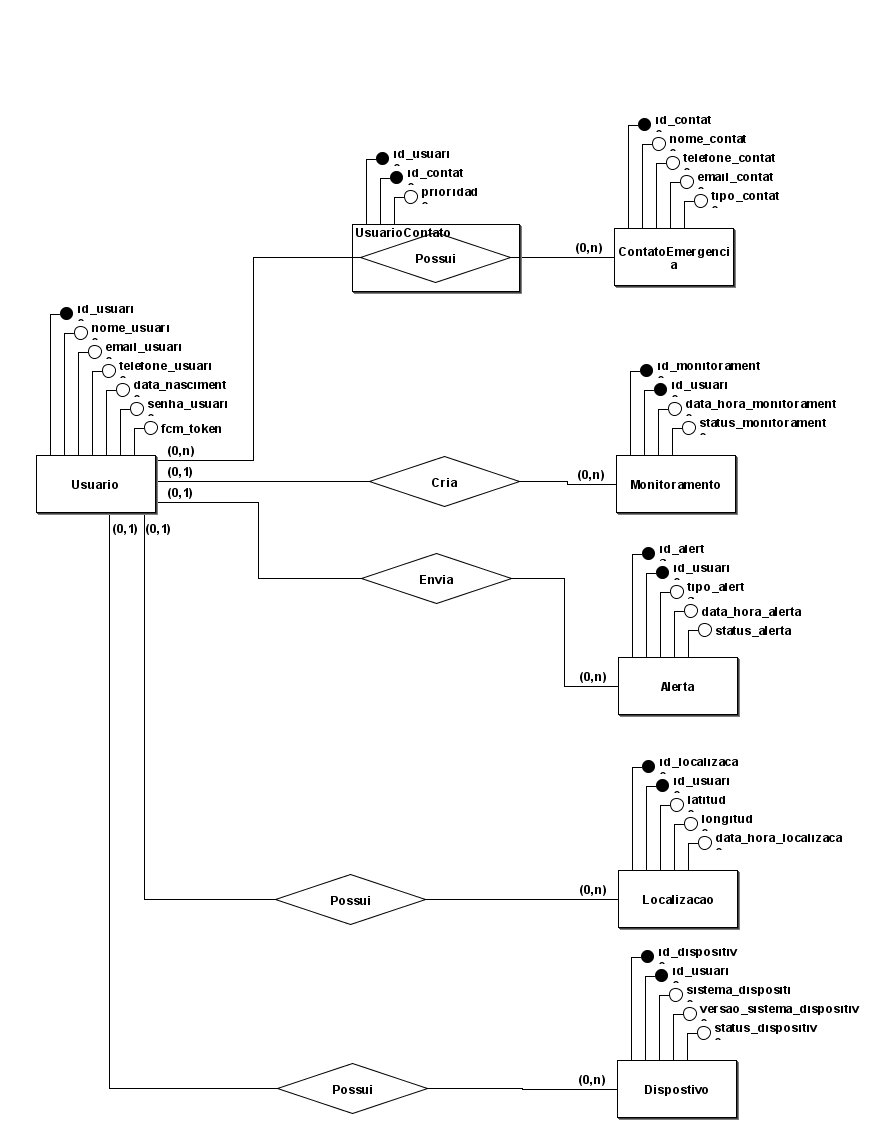
\includegraphics[scale=0.5]{imagens/modelo_entidade_relacionamento.png}
\end{center}
\legend{Fonte: Elaborado pelos autores.}
\end{figure}

A Figura~\ref{fig_der} apresenta o Diagrama Entidade-Relacionamento (DER), evidenciando as entidades, atributos e relacionamentos implementados no banco de dados.

\begin{figure}[H]
\caption{\label{fig_der}Diagrama Entidade-Relacionamento do sistema Linha Vital.}
\begin{center}
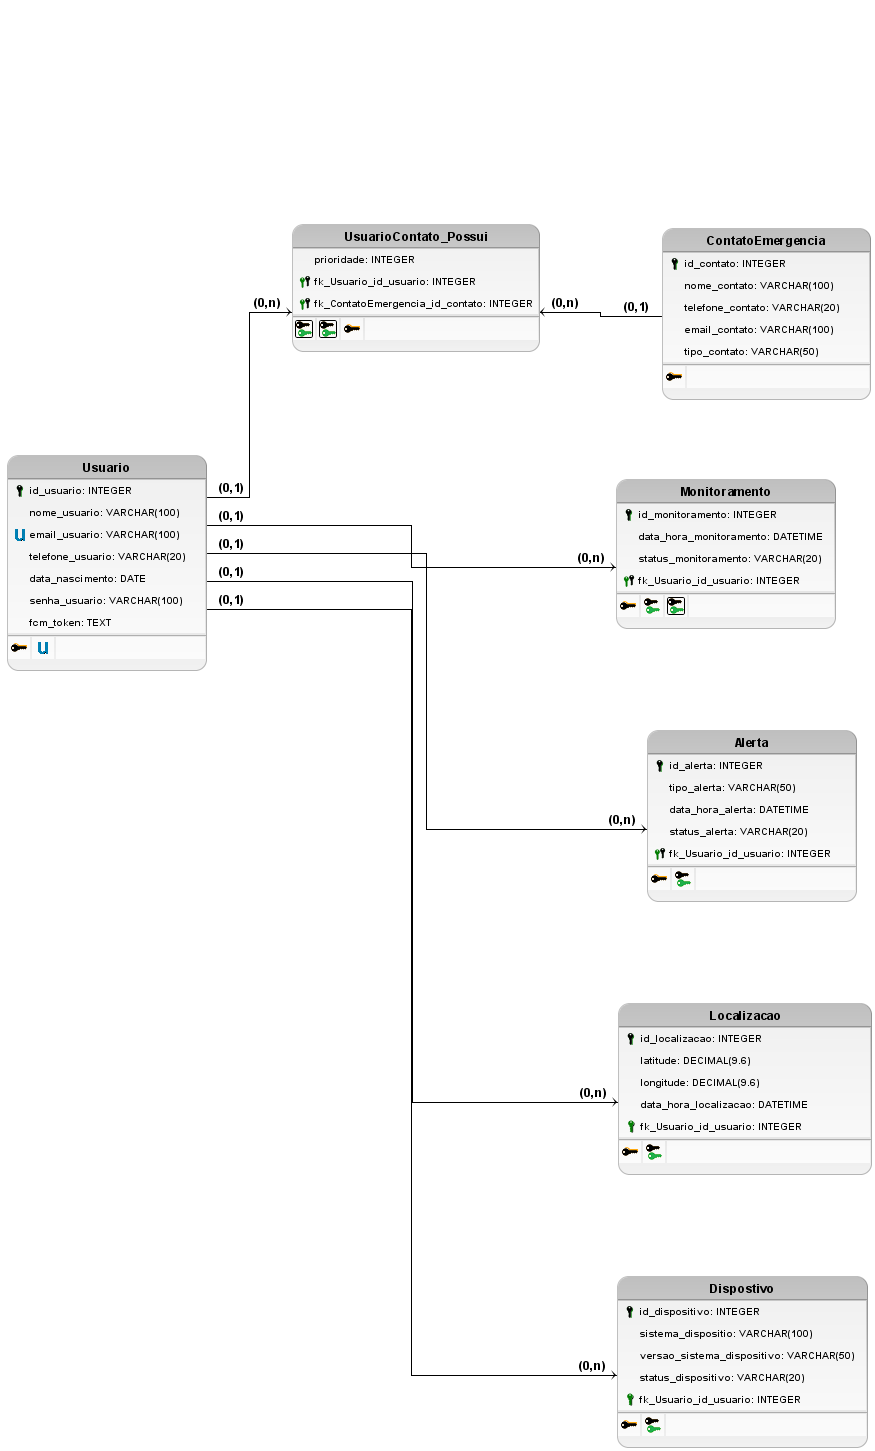
\includegraphics[scale=0.5]{imagens/diagrama_entidade_relacionamento.png}
\end{center}
\legend{Fonte: Elaborado pelos autores.}
\end{figure}

\subsection{Dicionário de Dados}

O dicionário de dados tem como finalidade documentar detalhadamente a estrutura do banco de dados utilizado pelo sistema Linha Vital, apresentando as tabelas, atributos, tipos de dados, restrições e descrições de cada elemento armazenado.

Essa documentação é fundamental para garantir a compreensão da modelagem adotada, facilitando atividades de desenvolvimento, manutenção e evolução da aplicação. Por meio do dicionário de dados, é possível identificar o papel de cada entidade no contexto do sistema, bem como os relacionamentos existentes entre elas.

Essa organização contribui para a integridade das informações armazenadas e para a padronização do acesso aos dados pelas diferentes camadas da aplicação.


O Quadro~\ref{quad_usuario} apresenta o dicionário de dados da entidade Usuario.

\begin{table}[H]
\caption{Dicionário de Dados da Entidade Usuario}
\label{quad_usuario}
\centering
\footnotesize

\begin{tabular}{|p{3cm}|p{2.5cm}|p{4cm}|p{5cm}|}
\hline
\textbf{Campo} & \textbf{Tipo} & \textbf{Restrição} & \textbf{Descrição} \\
\hline

id\_usuario & INTEGER & PK & Identificador único do usuário. \\
\hline

nome\_usuario & VARCHAR(100) & NOT NULL & Nome completo do usuário. \\
\hline

email\_usuario & VARCHAR(100) & UNIQUE, NOT NULL & Endereço de e-mail utilizado para autenticação. \\
\hline

telefone\_usuario & VARCHAR(20) & NOT NULL & Telefone principal do usuário. \\
\hline

data\_nascimento & DATE & NOT NULL & Data de nascimento do usuário. \\
\hline

senha\_usuario & VARCHAR(100) & NOT NULL & Senha criptografada do usuário. \\
\hline

fcm\_token & TEXT & NULL & Token utilizado para envio de notificações push. \\
\hline

\end{tabular}

\normalsize

\legend{Fonte: Elaborado pelos autores.}
\end{table}

O Quadro~\ref{quad_contato} apresenta o dicionário de dados da entidade ContatoEmergencia.

\begin{table}[H]
\caption{Dicionário de Dados da Entidade ContatoEmergencia}
\label{quad_contato}
\centering
\footnotesize

\begin{tabular}{|p{3cm}|p{2.5cm}|p{4cm}|p{5cm}|}
\hline
\textbf{Campo} & \textbf{Tipo} & \textbf{Restrição} & \textbf{Descrição} \\
\hline

id\_contato & INTEGER & PK & Identificador único do contato. \\
\hline

nome\_contato & VARCHAR(100) & NOT NULL & Nome do contato de emergência. \\
\hline

telefone\_contato & VARCHAR(20) & NOT NULL & Número telefônico do contato. \\
\hline

email\_contato & VARCHAR(100) & NULL & Endereço de e-mail do contato. \\
\hline

tipo\_contato & VARCHAR(50) & NOT NULL & Tipo do contato (emergência, confiança, familiar etc.). \\
\hline

\end{tabular}

\normalsize

\legend{Fonte: Elaborado pelos autores.}
\end{table}

\begin{table}[H]
\caption{Dicionário de Dados da Entidade UsuarioContato\_Possui}
\label{quad_usuario_contato}
\centering
\footnotesize

\begin{tabular}{|p{5,2cm}|p{2cm}|p{2.5cm}|p{4,8cm}|}
\hline
\textbf{Campo} & \textbf{Tipo} & \textbf{Restrição} & \textbf{Descrição} \\
\hline

fk\_Usuario\_id\_usuario & INTEGER & PK, FK & Referência ao usuário. \\
\hline

fk\_ContatoEmergencia\_id\_contato & INTEGER & PK, FK & Referência ao contato de emergência. \\
\hline

prioridade & INTEGER & NOT NULL & Ordem de acionamento dos contatos em situações de emergência. \\
\hline

\end{tabular}

\normalsize

\legend{Fonte: Elaborado pelos autores.}
\end{table}

O Quadro~\ref{quad_monitoramento} apresenta o dicionário de dados da entidade Monitoramento.

\begin{table}[H]
\caption{Dicionário de Dados da Entidade Monitoramento}
\label{quad_monitoramento}
\centering
\footnotesize

\begin{tabular}{|p{4.0cm}|p{2.5cm}|p{2.5cm}|p{5.5cm}|}
\hline
\textbf{Campo} & \textbf{Tipo} & \textbf{Restrição} & \textbf{Descrição} \\
\hline

id\_monitoramento & INTEGER & PK & Identificador do monitoramento. \\
\hline

data\_hora\_monitoramento & DATETIME & NOT NULL & Data e hora do registro do monitoramento. \\
\hline

status\_monitoramento & VARCHAR(20) & NOT NULL & Estado atual do monitoramento. \\
\hline

fk\_Usuario\_id\_usuario & INTEGER & FK & Usuário relacionado ao monitoramento. \\
\hline

\end{tabular}

\normalsize

\legend{Fonte: Elaborado pelos autores.}
\end{table}

O Quadro~\ref{quad_alerta} apresenta o dicionário de dados da entidade Alerta.

\begin{table}[H]
\caption{Dicionário de Dados da Entidade Alerta}
\label{quad_alerta}
\centering
\footnotesize

\begin{tabular}{|p{4.0cm}|p{2.5cm}|p{2.5cm}|p{5.5cm}|}
\hline
\textbf{Campo} & \textbf{Tipo} & \textbf{Restrição} & \textbf{Descrição} \\
\hline

id\_alerta & INTEGER & PK & Identificador único do alerta. \\
\hline

tipo\_alerta & VARCHAR(50) & NOT NULL & Categoria do alerta gerado. \\
\hline

data\_hora\_alerta & DATETIME & NOT NULL & Data e hora do acionamento. \\
\hline

status\_alerta & VARCHAR(20) & NOT NULL & Situação atual do alerta. \\
\hline

fk\_Usuario\_id\_usuario & INTEGER & FK & Usuário associado ao alerta. \\
\hline

\end{tabular}

\normalsize

\legend{Fonte: Elaborado pelos autores.}
\end{table}

O Quadro~\ref{quad_localizacao} apresenta o dicionário de dados da entidade Localizacao.

\begin{table}[H]
\caption{Dicionário de Dados da Entidade Localizacao}
\label{quad_localizacao}
\centering
\footnotesize

\begin{tabular}{|p{4.0cm}|p{2.5cm}|p{2.5cm}|p{5.5cm}|}
\hline
\textbf{Campo} & \textbf{Tipo} & \textbf{Restrição} & \textbf{Descrição} \\
\hline

id\_localizacao & INTEGER & PK & Identificador da localização registrada. \\
\hline

latitude & DECIMAL(9,6) & NOT NULL & Latitude da posição do usuário. \\
\hline

longitude & DECIMAL(9,6) & NOT NULL & Longitude da posição do usuário. \\
\hline

data\_hora\_localizacao & DATETIME & NOT NULL & Data e hora da coleta da localização. \\
\hline

fk\_Usuario\_id\_usuario & INTEGER & FK & Usuário associado ao registro. \\
\hline

\end{tabular}

\normalsize

\legend{Fonte: Elaborado pelos autores.}
\end{table}

\section{Duração e Cronograma}

A duração do projeto Linha Vital foi estimada considerando as atividades necessárias para análise, desenvolvimento, testes, documentação e implantação da solução. Como a equipe adotou a metodologia Scrum, o planejamento foi estruturado em ciclos iterativos e incrementais, permitindo que as funcionalidades fossem desenvolvidas e validadas de forma progressiva.

Diferentemente de abordagens tradicionais, o cronograma não foi definido por meio de fases rígidas e sequenciais, mas sim por sprints organizadas de acordo com as prioridades do projeto e a evolução das funcionalidades implementadas. Essa abordagem proporcionou maior flexibilidade para adequação de requisitos, correção de problemas identificados durante o desenvolvimento e adaptação às necessidades do produto.

\subsection{Análise da duração do projeto}

A estimativa de duração do projeto considerou a divisão das atividades em etapas de levantamento de requisitos, modelagem, implementação, integração, testes e documentação. Cada uma dessas etapas foi distribuída ao longo de sprints planejadas pela equipe, permitindo entregas incrementais e acompanhamento contínuo da evolução do sistema.

A utilização de ciclos curtos de desenvolvimento favoreceu a identificação antecipada de riscos e a validação constante das funcionalidades implementadas, reduzindo retrabalho e contribuindo para a qualidade do produto final.

O detalhamento das atividades executadas, bem como sua distribuição ao longo das sprints, encontra-se representado no roadmap de desenvolvimento elaborado pela equipe, apresentado posteriormente neste trabalho.